\chapter{Tutorial and examples}
\label{app:tuto}

The \proj{OsmocomBB} website describes every step needed to run the
software, but an overview is given here as well~\cite{osmocombb_2015}.
This section also explains how to apply the patches developed for this
thesis and test the various new commands.

\section{Installation}

The installation consists of five steps: installing the dependencies
needed to compile the software, compiling and installing the libosmocore
library, installing a toolchain to compile the firmware for the ARM
baseband processor, applying the patch created for this thesis, and
compiling OsmocomBB.

\subsection{Dependencies}

On a Debian based system, the dependencies can be installed using:

      \begin{lstlisting}[language=bash, numbers=left,
      basicstyle=\footnotesize, breaklines=true, frame=single]
sudo apt-get install libtool shtool automake autoconf git pkg-config make gcc libpcsclite-dev
      \end{lstlisting}

\subsection{Libosmocore}

Libosmocore contains the common code between the various \proj{Osmocom}
projects.

      \begin{lstlisting}[language=bash, numbers=left,
      basicstyle=\footnotesize, breaklines=true, frame=single]
git clone git://git.osmocom.org/libosmocore.git
cd libosmocore/
autoreconf -i
./configure
make
sudo make install
cd ..
      \end{lstlisting}

\subsection{GNU toolchain for ARM}

This toolchain is needed to compile the code running on the ARM baseband
processor.

      \begin{lstlisting}[language=bash, numbers=left,
      basicstyle=\footnotesize, breaklines=true, frame=single]
mkdir toolchain
cd toolchain
wget bb.osmocom.org/trac/raw-attachment/wiki/GnuArmToolchain/gnu-arm-build.2.sh
chmod +x gnu-arm-build.2.sh

#GCC 4.5.2 can not be compiled with texinfo 5
wget https://gitlab.com/francoip/thesis/raw/public/patch/gnu-arm-build-texinfo5.patch
wget https://gitlab.com/francoip/thesis/raw/public/patch/gcc-texinfo5.patch
patch < gnu-arm-build-texinfo5.patch #The patch gcc-texinfo5.patch was adapted from Marcello Pogliani <pogliamarci@hotmail.it>.

sudo apt-get install build-essential libgmp3-dev libmpfr-dev libx11-6 libx11-dev texinfo flex bison libncurses5 \
  libncurses5-dbg libncurses5-dev libncursesw5 libncursesw5-dbg libncursesw5-dev zlibc zlib1g-dev libmpfr4 libmpc-dev

mkdir build install src
cd src/
wget http://ftp.gnu.org/gnu/gcc/gcc-4.5.2/gcc-4.5.2.tar.bz2
wget http://ftp.gnu.org/gnu/binutils/binutils-2.21.1a.tar.bz2
wget ftp://sources.redhat.com/pub/newlib/newlib-1.19.0.tar.gz
cd ..
./gnu-arm-build.2.sh

export PATH=$PATH:<YOURPATH>/install/bin
      \end{lstlisting}
      \iffalse $ \fi

\subsection{OsmocomBB and patches}

Finally, compiling the OsmocomBB software and applying the various
patches created for this thesis can be done easily.

      \begin{lstlisting}[language=bash, numbers=left,
      basicstyle=\footnotesize, breaklines=true, frame=single]
git clone git://git.osmocom.org/osmocom-bb.git
cd osmocom-bb
git pull --rebase
wget https://gitlab.com/francoip/thesis/raw/public/patch/thesis.patch
wget https://gitlab.com/francoip/thesis/raw/public/patch/aftenposten.patch
patch -p1 < thesis.patch
patch -p1 < aftenposten.patch
cd src
make
      \end{lstlisting}

\section{Usage of \prog{mobile}}

Compatible phones and cables are listed on the project website. A
picture of the running setup is shown in \fref{fig:C118}.

     \begin{figure}[h]
        \centering
        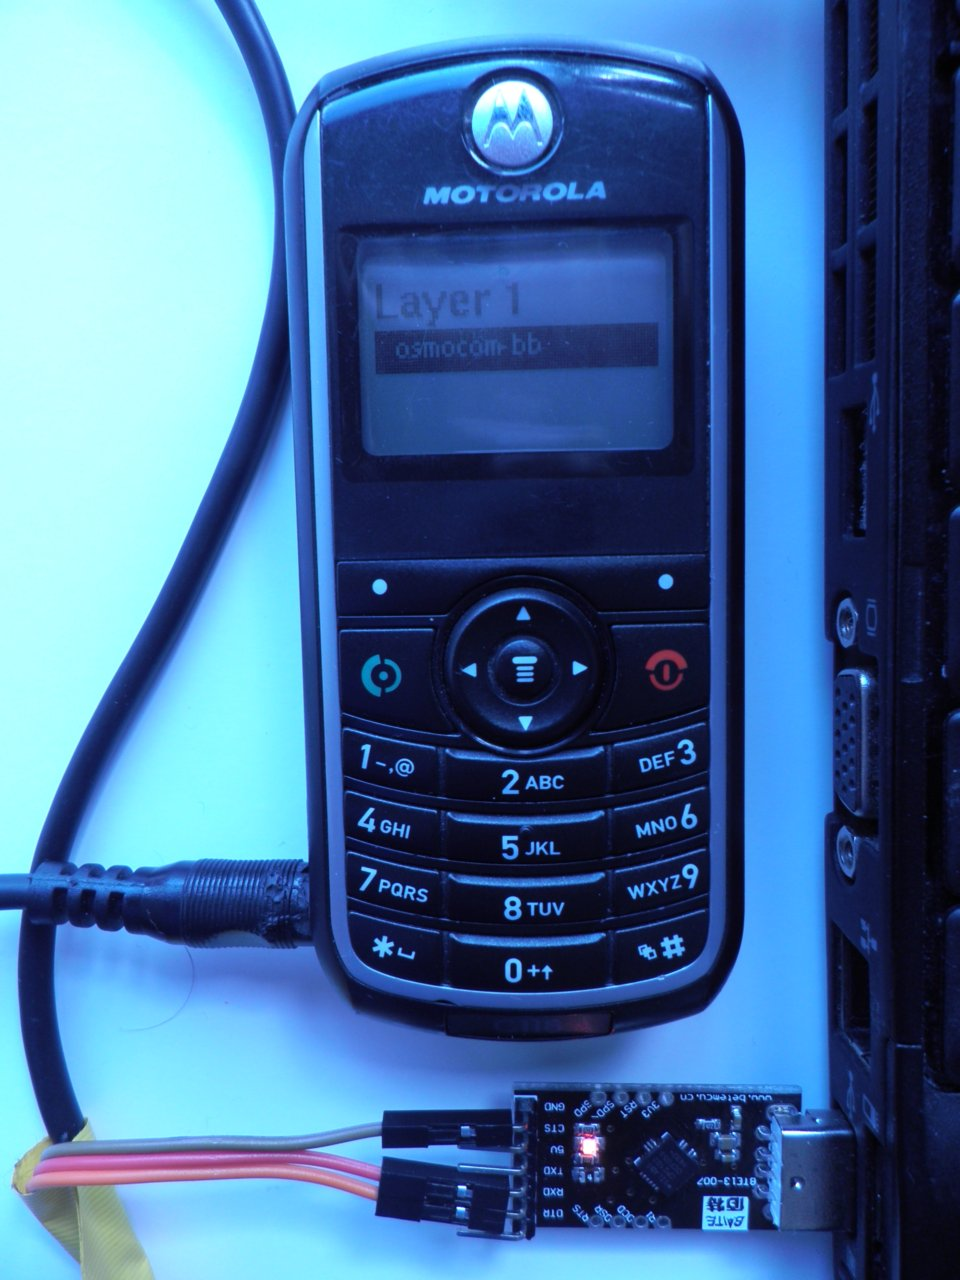
\includegraphics[width=0.5\textwidth]{C118}
        \caption{Motorola C118 connected to a computer with a CP2102 USB
        to serial converter.}
        \label{fig:C118}
      \end{figure}

Four steps are needed to use the \prog{mobile} application when the
phone is connected to the computer using the appropriate cable. The first
step is to start Wireshark:
      \begin{lstlisting}[language=bash, numbers=left,
basicstyle=\footnotesize, breaklines=true, frame=single]
nc -u -l -p 4729 > /dev/null & wireshark -k -i lo -f 'port 4729'
      \end{lstlisting}

The second step is to load the firmware on the phone by starting the
\prog{osmocon} application in a second terminal, then by pressing the
power button on the phone. In this case, the command is:

      \begin{lstlisting}[language=bash, numbers=left,
basicstyle=\footnotesize, breaklines=true, frame=single]
sudo host/osmocon/osmocon -m c123xor -p /dev/ttyUSB0 target/firmware/board/compal_e88/layer1.compalram.bin
      \end{lstlisting}

The third step is to start the \prog{mobile} application. In a third
terminal. If the \prog{mobile} application was started with the \code{-i
127.0.0.1} argument, all the layer 3 messages are readable in
\proj{Wireshark} if it is listening on the \code{localhost}.

      \begin{lstlisting}[language=bash, numbers=left,
basicstyle=\footnotesize, breaklines=true, frame=single]
sudo host/layer23/src/mobile/mobile -i 127.0.0.1 
      \end{lstlisting}

The last step is to connect to the application interface using
\prog{telnet} in a new termilal:
      \begin{lstlisting}[language=bash, numbers=left,
basicstyle=\footnotesize, breaklines=true, frame=single]
telnet localhost 4247
      \end{lstlisting}

Then, commands can be sent to the software through this interface. For
example the \prog{dos camp} command described in
\Sref{sec:rachell_demo}. All the commands have built-in help integrated
in the interface.

      \begin{lstlisting}[numbers=left,
basicstyle=\footnotesize, breaklines=true, frame=single]
OsmocomBB> en
OsmocomBB# dos camp 1 242 01
      \end{lstlisting}

\iffalse
\subsection{Sending a silent SMS message}

This is an example of the modified \prog{mobile} application usage to
send a silent SMS message. These commands need to be written in the
\prog{telnet} prompt. If the \prog{mobile} application was started with
the \code{-i 127.0.0.1} argument, all the layer 3 messages are readable
in \proj{Wireshark} if it is listening on the \code{localhost}.

      \begin{lstlisting}[numbers=left,
basicstyle=\footnotesize, breaklines=true, frame=single]
OsmocomBB> en
OsmocomBB# silent 1 1
OsmocomBB# sms 1 +47123456 Example of silent SMS message
      \end{lstlisting}
\fi

\section{Usage of \prog{cell\_log}}

The \prog{mobile} application is not the only one available. The
\prog{cell\_log} application can be used to determine the most suitable
ARFCN in the vicinity. The following commands can be used after the two
first steps described in the previous section.

      \begin{lstlisting}[language=bash, numbers=left,
basicstyle=\footnotesize, breaklines=true, frame=single]
cd osmocom-bb
sudo src/host/layer23/src/misc/cell_log -l /tmp/cell_log
less /tmp/cell_log
      \end{lstlisting}

\section{Using the \code{burst\_ind} branch}

To use \proj{OsmocomBB} as a passive listener, as explained in
\Sref{sec:passive_listener}, the \code{burst\_ind} branch needs to be
used. This can be done using the following commands.

      \begin{lstlisting}[language=bash, numbers=left,
basicstyle=\footnotesize, breaklines=true, frame=single]
git clone git://git.osmocom.org/osmocom-bb.git burst_ind
cd burst_ind
git checkout sylvain/burst_ind
git pull --rebase
cd src
echo "#define I_HAVE_A_CP210x" >> host/osmocon/osmocon.c
make
      \end{lstlisting}

To use this branch, a CP2102 cable is needed. The \prog{ccch\_scan}
application in this branch is intended as a demonstration of its
capabilities.

      \begin{lstlisting}[language=bash, numbers=left,
basicstyle=\footnotesize, breaklines=true, frame=single]
cd burst_ind
sudo src/host/layer23/src/misc/ccch_scan -a ARFCN
      \end{lstlisting}
